\documentclass[letterpaper,10pt,conference]{ieeeconf}
\IEEEoverridecommandlockouts
\overrideIEEEmargins

\usepackage[utf8]{inputenc}
\usepackage[T1]{fontenc}

\usepackage{xcolor}
\usepackage{xspace}

%these commands are used to make ieeeconf play nice with amsthm
\makeatletter
\let\IEEEproof\proof
\let\IEEEendproof\endproof
\let\proof\@undefined
\let\endproof\@undefined
\makeatother

\usepackage{amsmath,amssymb,amsthm}
\usepackage{graphicx,url}
\usepackage{microtype}
\usepackage{cleveref}
\usepackage{csquotes}
\usepackage{siunitx}
\usepackage{bm}

\usepackage{algpseudocode}
\usepackage{algorithm}
\usepackage{float}

\usepackage[style=ieee]{biblatex}
\addbibresource{references.bib}

\renewcommand{\vec}[1]{\bm{#1}}
\newcommand{\R}{{\mathbb{R}}}
\DeclareMathOperator{\diag}{diag}
\DeclareMathOperator{\atantwo}{atan2}


\urldef{\you}\url{astoecke@uwaterloo.ca}

\title{Bug Algorithms using Neural Networks}
\date{August 7th, 2017}
\author{Andreas Stöckel\thanks{}
  \thanks{The author is with the Cheriton School of Computer Science and the Centre for Theoretical Neuroscience, University of Waterloo, Waterloo ON, N2L 3G1
    Canada  (\you)}}


\begin{document}

\maketitle

\begin{abstract}
In robotic and biological agents alike, path planning is often restricted to local, sensor-based information. In cases where self-localisation and mapping techniques are infeasible, a resource-efficient alternative relying on few sensors and minimal memory is the family of so called \emph{bug algorithms}. Despite their name, bug algorithms are not biologically motivated and relatively abstract. Here, I present a prototypical implementation of the \emph{Bug 0} and \emph{Bug 2} algorithms as a biologically constrained spiking neural network built using the Neural Engineering Framework (NEF). Simulations show that the resulting neurally controlled agents successfully navigate simple environments. Failed navigation attempts in complex environments illustrate challenges arising when implementing relatively abstract algorithms as neural networks.
\end{abstract}

\section{Introduction}

Navigation---travelling from a current location in space to a possibly hidden goal---is fundamental to both animal and mobile robot behaviour. Animals rely on navigation to forage food sources, while analogously mobile robots may need to return to a charging station whenever their battery runs low. Especially in small animals such as insects path planning is restricted to local, sensor-based information and supposedly little memory. Likewise, autonomous robots may be restricted to local information whenever it is desirable to design energy- and cost-efficient systems with few computational resources, rendering accumulation of global information over time, e.g.~simultaneous localization and mapping (SLAM, \cite{thrun2002probabilistic}), infeasible.

\emph{Bug algorithms} are a class of sensor-based navigation algorithms proposed by Lumelsky and Stepanov in 1987 \cite{lumelsky1987path}. Extending basic obstacle-following and goal-directed behaviours, these algorithms guarantee to guide an agent along a path from start to goal exactly if such a path exists. However, being of an abstract nature, it is non-trivial to implement these algorithms on a physical robot platform, and even more so when using a biologically constrained computing substrate. While the original authors were probably inspired by biology, they make no claim whatsoever of biological plausibility. Still, the simplicity of the algorithms poses the question whether they actually could be a viable strategy for animals or, in a broader sense, agents performing biologically constrained computations using spiking neural networks.

In the context of path planning with incomplete information, bug algorithms were originally proposed to show that provable strategies exist, i.e.~one can prove that the strategy will actually find a solution exactly if a solution exists. Only heuristics---algorithms without this property---had been previously proposed for this problem. Improved versions of the algorithms have been published, such as \emph{VisBug} \cite{lumelsky1990incorporating}, \emph{DistBug} \cite{kamon1997sensorybased}, and \emph{TangentBug} \cite{kamon1998tangentbug} which incorporate range sensor information in order to decide when to switch between behaviours. A comprehensive overview of bug algorithms is given in \cite{lavalle2006planning}. For the sake of simplicity I focus on the original bug algorithms, yet techniques similar to those presented here should be applicable to more advanced models as well.

Building biologically constrained models of neural systems and cognitive tasks is a central aim of computational neuroscience and can be traced back to models of spiking behaviour of single neurons presented in the 1950s \cite{hodgkin1952quantitative}. The central challenge is to combine individual model neurons in such a way that the network fulfills a desired task, that is to build \emph{functional} networks. In recent years multiple modelling frameworks have been proposed, aiming at simplifying the construction of functional neural networks, while at the same time accounting for empirical neurobiological data. According to \cite{komer2016unified}, approaches include a technique by Denève et~al.~for modelling dynamical systems as neural networks \cite{martin2013predictive}, detailed reproduction of biological networks as strived for in the Human Brian Project \cite{markram2012human}, and the Neural Engineering Framework (NEF), which constructs neural networks from mathematical descriptions \cite{eliasmith2003neural}.

The ability to construct functional spiking neural networks is not only interesting from the perspective of neuroscience alone. For engineers, providing spiking neural network implementations of mobile robot control algorithms---a field also called \emph{neurorobotics}---enables their execution on analogue neuromorphic hardware systems, which promise magnitudes improved power-efficiency compared to traditional digital computers \cite{boahen2017neuromorph}.

The contribution of this paper is to provide a prototypical implementation of two bug algorithms as spiking neural network using the NEF. In particular, I explore an implementation of a network which provides discrete state transitions, which is an important building block in the bug algorithm implementation. For evaluation purposes, I employ a custom robot simulator to compare the behaviour of the neural implementation to a traditionally implemented reference.

The remainder of this paper is structured as follows. In \Cref{sec:background} I give an overview of both bug algorithms and the NEF, followed by a detailed description of the implementation in \Cref{sec:methods}. In \Cref{sec:experiments} I briefly present a set of experiments and their results, followed by a short discussion. \Cref{sec:conclusion} concludes this work by summarizing the main results and discussing future research directions.

\section{Background Material}
\label{sec:background}

Here, I review the two bug algorithms implemented in this paper and summarize the basic ideas underlying the NEF. Note that the description of Bug algorithms is mainly adapted from \cite{lumelsky1987path,lavalle2006planning,bullo2016lectures}, whereas detailed treatments of the NEF and its applications can be found in \cite{eliasmith2003neural,eliasmith2012large,stewart2012neural,eliasmith2013build}.

\subsection{Bug Algorithms}
\label{sec:bug_algorithms}

Bug algorithms solve the task of navigating from a start location $\vec p_\mathrm{start}$ to a goal location $\vec p_\mathrm{goal}$ in a two-dimensional environment featuring polygonal obstacles. It is assumed that the robot is holonomic, point-shaped (i.e.~it has no physical extent), and senses its current location $\vec p$, as well as the goal location---or equivalently, and assuming the robot has an orientation, the robot knows the direct-line distance, as well as the absolute (with respect to the world reference frame) and relative (with respect to its own orientation) angle to the goal. Furthermore, the algorithms assume the robot has a contact sensor detecting obstacle collisions. The robot supports two basic behaviours, namely driving in a straight line towards the goal and closely following an obstacle outline. As a major limitation, its memory system is limited and capable of storing few distances and angles only.

The basic algorithm in the bug family is Bug 0 \cite{bullo2016lectures}:
\begin{algorithmic}[1]
	\While{not at goal}
	\State{move towards the goal}
	\If{hit an obstacle}
	\While{not able to move towards the goal}
	\State{follow obstacle boundary \emph{counter clock wise}}
	\EndWhile
	\EndIf
	\EndWhile
\end{algorithmic}
Note that this algorithm does not guarantee finding a path from start to goal. Some obstacle topologies will send the agent around in circles, and since it has no memory, the robot has no chance of ever exiting one of these cycles.

Two of the originally proposed solutions to this problem are the Bug 1 and Bug 2 algorithms. Bug 1 circumnavigates the entire obstacle outline, tracks the point with the minimum distance to the goal, and continues to drive towards the goal at this point. Bug 2 avoids circumnavigating the entire obstacle by driving towards the goal whenever the robot crosses the start-goal line and the current distance to the goal is smaller than the distance to the goal upon hitting the obstacle, or, expressed in terms of the absolute direction sensor:
\begin{algorithmic}[1]
	\State{$\alpha \gets$ goal direction}
	\While{not at goal}
	\State{move towards the goal}
	\If{hit an obstacle}
	\State{$d_\mathrm{hit} \gets$ distance to goal}
	\While{distance to goal $\geq d_\mathrm{hit}$ \textbf{or}\\\hspace{2cm}goal direction $\neq \alpha$}
	\State{follow obstacle boundary}
	\EndWhile						
	\EndIf
	\EndWhile
\end{algorithmic}
Note that Bug 2 does not always perform better than Bug 1 in terms of the total path length, but in general the trajectory produced by Bug 2 seems more sensible to the human observer.
In the following I focus on a neural implementation of the Bug 0 and Bug 2 algorithms. Due to time constraints, I will not implement Bug 1---however, since both Bug 1 and 2 make use of the same basic sensor, state transition, and memory system, the techniques for the realization of Bug 2 could be transferred to an implementation of Bug 1	.


\subsection{The Neural Engineering Framework (NEF)}

The NEF \cite{eliasmith2003neural} is a systematic approach to modelling spiking neural networks from a mathematical description. To this end, the NEF relies on three key principles: \emph{(i)} ensembles of neurons represent vectors $\vec x \in \R^d$, \emph{(ii)} connections between ensembles compute functions $f(\vec x)$, and \emph{(iii)} recurrent connections realize time-dynamics $\dot {\vec x} = f(\vec x) + g(\vec y)$. While the NEF itself imposes relatively few restrictions on the neuron model, I model each neuron in the network as \emph{leaky integrate and fire} (LIF) neuron
\begin{align*}
	\tau_\mathrm{RC} \cdot \dot u(t) &= J - u(t)\,, \\
	u(t') &\gets 0 \, \forall t' \in [t, t + \tau_\mathrm{ref}]\text{ if } u(t) \geq 1 \,,
\end{align*}
where $\tau_\mathrm{RC}$ is the membrane time constant, $u$ is the membrane potential, and $J$ is the input current injected into the membrane. Once the $u$ reaches a certain threshold potential, an output spike is issued and $u$ is clamped to zero for the duration of the so called refractory period $\tau_\mathrm{ref}$.

Assume an ensemble of $n$ neurons receives input from $m$ pre-synaptic neurons. Then, the input current vector $\vec J \in \mathbb{R}^n$ is defined over time as
\begin{align}
	\vec J(t)
		&= \diag(\vec \alpha) W \vec a(t) + \vec J_\mathrm{bias}
	\label{eqn:j_w}
\end{align}
where $\vec \alpha, \vec J_\mathrm{bias} \in \R^n$ are vectors of scalar gain factors and offsets, $W \in \mathbb{R}^{m \times n}$ is a weight matrix wherein $(W)_{ij}$ describes the connection weight between the $i$th pre-synaptic and the $j$th post-synaptic neuron, and $\vec a(t) \in \mathbb{R}^m$ is a function describing the activity of the pre-synaptic population
\begin{align*}
	(\vec a(t))_i &= \int_{-\infty}^\infty \sum_k \delta(t - t' - t^\mathrm{spike}_{ik}) \cdot H(t') \,\mathrm{d}t'\,.
\end{align*}
Here, $\delta(t)$ is a Dirac-pulse, $H$ is a convolution kernel describing synaptic dynamics, and $t^\mathrm{spike}_{ik}$ is the time of the $k$th output spike of the $i$th presynaptic neuron.

The core idea of the NEF is to factorise the weights $W$ into of encoding and decoding vectors, turning \Cref{eqn:j_w} into
\begin{align*}
	\vec J(t) &= \diag(\vec \alpha) E D \vec a(t) + \vec J_\mathrm{bias} \,.
\end{align*}
The $d$-dimensional encoding vectors in $E \in \R^{n \times d}$ are randomly selected for each of the $n$ neurons in an ensemble. Given a low-dimensional vector $\vec x \in \R^d$, the operation $E \vec x$ projects $\vec x$ into an $n \gg d$ dimensional neural activity space, while the decoding matrix $D \in \R^{d \times m}$ decodes $d$-dimensional representations from the $m$-dimensional pre-synaptic activity. Measuring steady-state pre-synaptic neural activities for a range of represented values $\vec x$, arranging them in a matrix $A$, and placing the desired decoded values $f(\vec x)$ in a matrix $Y$, we can find the decoding matrix $D^f$ calculating $f$ using simple least-squares regression
\begin{align*}
	Y \overset{!}= D^f A \Rightarrow D^f \approx Y A^T (A A^T + \sigma I)^{-1} \,,
\end{align*}
where $\sigma$ is a regularization factor. This method is similar to the kernel method \cite{hofmann2008kernel}. Low-dimensional functions $g$ are randomly and non-linearly (with the neurons being the non-linearity) projected into a high-dimensional function space (defined by neural activity $\vec a$ and the encoding matrix $E$), which in turn is linearly---and approximately---projected onto our desired function $f$ by $D$. Empirical analysis shows that this approximation works best for functions which can be represented with low-order Legendre polynomials. The approximation error decreases as a function in $\mathcal{O}(1 / \sqrt{n})$.

Recurrent connections on a single neuron ensemble allow to implement arbitrary dynamics $\dot {\vec x} = f(\vec x) + g(\vec y)$, where $\vec x$ is the value represented by the neuron ensemble and $\vec y$ is an input value represented by another ensemble. Assuming $H$ is a first-order exponential low-pass filter with time-constant $\tau_\mathrm{syn}$, one can show that the functions $f'$ and $g'$ that must be decoded to realize this system are
\begin{align*}
	f'(\vec x) &= \tau_\mathrm{syn} \, f(\vec x) + \vec x \,, & g'(\vec y) = \tau_\mathrm{syn} \, g(\vec y) \,.
\end{align*}

To summarize, given the NEF, building functional spiking neural networks can be distilled into defining vectorial quantities, functions transforming these quantities, and dynamics evolving over time. Given the number of neurons representing each quantity, as well as neuron parameters $E$, $\vec \alpha$, and $\vec J_\mathrm{bias}$, we can compute ensemble activities over $\vec x$ and optimize for decoders $D$, resulting in connection weights $W = ED$. Conveniently, this process is implemented in a Python package called Nengo\footnote{Software available at \url{https://www.nengo.ai/}} \cite{bekolay2014nengo}, which is used  in the following for both neural network description and simulation.

\section{Methods}
\label{sec:methods}

This section focuses on the bug algorithm implementation. I first introduce the robot simulator and a mathematical description of the basic robot behaviours, leading to the network topology implementing the Bug 0 behaviour. I then use a neural state transition sub-network to extend this basic variant to the Bug 2 algorithm 

\subsection{Robot Simulator}


\begin{figure}
	\centering
	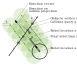
\includegraphics{media/robot_environment.pdf}
	\caption{Illustration of the robot movement model and collision queries. Obstacle points (plum) are queried (green) along three rays parallel to the direction vector. On collision, the direction vector is projected onto the obstacle outline orientation and movement continues in that direction.}
	\label{fig:robot_environment}
\end{figure}

The robot simulator has been specifically implemented for this project. In contrast to the assumptions in the algorithm description, the virtual robot is disc-shaped with radius $r = \SI{0.15}{\centi\meter}$ and has a non-holonomic drive controlled by a steering vector $\vec v = (v_x, v_y)$ encoding both the desired change in orientation $\dot \alpha \propto \atantwo(x_y, v_x)$, as well as the velocity $\| \dot {\vec p} \| = \|\vec v\|$. In addition to the sensors listed in the theoretical description of the bug algorithms, the robot is equipped with a low-dimensional omnidirectional range sensor for obstacle outline following. Absolute and relative goal directions are represented as two-dimensional unit vectors.

The environment is read from a low-resolution ASCII bitmap. Obstacle outlines are vectorized into polygons, simplified, and subdivided with a maximum distance $\epsilon$ between vertices. Vertices are stored in a $k$-d tree \cite{bentley1975multidimensional} for logarithmic lookup time in collision queries. Ray-polygon intersections are performed by subdividing the ray into vertices with $\epsilon$ distance, querying obstacle vertices within an $\epsilon$-ball centred at each ray vertex, and calculating ray-line intersection between the ray and the polygon segments associated to each obstacle vertex. Robot motion is simulated in discrete $\SI{10}{\milli\second}$ timesteps.

As sketched in \Cref{fig:robot_environment}, collision detection is performed by sending three parallel rays along the desired robot path and performing corresponding ray-polygon intersection queries. Upon collision, the robot centre is set to the closest possible distance $d$ to the obstacle outline, as calculated by
\begin{align*}
	d = r \cdot \left(1 - \frac{|\langle \vec d, \vec o \rangle |}{\|\vec d\| \cdot \|\vec o\|} \right)^{-\frac{1}2} \,,
\end{align*}
where $\vec d$ and $\vec o$ are the current movement direction and obstacle orientation. The robot then continues along the obstacle, by projecting the direction onto the outline
\begin{align*}
	\vec d' = \frac{\langle \vec d, \vec o \rangle \cdot \vec o}{\| \vec o \|} \,.
\end{align*}
Physically this corresponds to having no friction between the robot and its environment, and allows sliding along obstacles.

In the simulator software, individual behavioural patterns are implemented as part of callback function invoked at each timestep, which transforms current sensor data and into a motor command $\vec v$. In the case of neural network controlled agents, the callback function feeds sensor data into the network, advances the Nengo simulation, and decodes the motor output from the network.

For evaluation purposes the simulator calculates the ground-truth shortest path (assuming a point robot) by constructing a visibility graph of the obstacle polygon corner points and start and goal points as outlined in \cite{bullo2016lectures}. The set of shortest paths between all start and goal points defined in the environment is obtained by repeated execution of Dijkstra's algorithm \cite{dijkstra1959note}.

\subsection{Basic Robot Behaviours}

As discussed above, the bug algorithms rely on the robot being capable of two basic behaviours: moving towards the goal in a straight line and closely following an obstacle outline. In the simulation framework presented above, the first behaviour can be trivially implemented by setting the motor command $\vec v$ to a vector proportional to the agent's relative goal direction vector. Note that in contrast to the algorithmic assumptions, the robot's trajectory will describe a curve instead of a straight line in most circumstances.

\begin{figure}
       \centering
       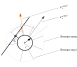
\includegraphics{media/robot_wall_following.pdf}
       \caption{Illustration of the range sensor used for wall following. Wall following is achieved by calculating a weighted sum of rotated sensor rays 
		(depicted: sensor ray $\vec r_i$ with the shortest distance $d_i$ rotated by $45^\circ$ and $90^\circ$). The depicted set of non-symmetric sensor orientations 
		was chosen to break symmetries causing the robot to get stuck at corners.}
       \label{fig:robot_wall_following}
\end{figure}

As outlined in \cite{yata1998wall}, the omnidirectional range sensor present on the virtual robot can be used to implement a wall following behaviour by moving perpendicular to the sensor ray with the shortest distance to the wall. Since the function $\arg\min_i d_i$ is only representable with high-order terms of the Legendre function basis, this algorithm is surprisingly hard to implement with few neurons in the NEF. To this end, I simplify the algorithm by calculating a weighted sum of the rotated sensor direction vectors, where rays corresponding to a smaller distance have quadratically greater weight. Furthermore, I rotate the ray vectors by $45^\circ$ instead of $90^\circ$, which forces the robot to move towards the obstacle and to slide along the wall upon collision. The final motor command $\vec v$ for the obstacle-following behaviour is given as
\begin{align*}
	\vec v = \sum_{i = 1}^n \left( 1 - \frac{d_i - r}{1 - r} \right)^2 \cdot \vec r_i^{\measuredangle 45^\circ} \,,
\end{align*}
where $n$ is the number of sensor rays, $d_i$ is the measured distance for the $i$th ray, $r$ is the robot radius, the one in the denominator corresponds to the maximum sensor range, and $\vec r_i^{\measuredangle 45^\circ}$ is the direction vector of the $i$th ray rotated by $45^\circ$ (see also \Cref{fig:robot_wall_following}). Importantly, due to finite rotation speed of the simulated robot, the robot will not always stay in contact with the obstacle outline. Especially when passing sharp corners, the presented strategy will cause the robot to overshoot before it moves back to the wall. Additionally, note that this algorithm implicitly causes the agent to move along the obstacle outline with a fixed rotational direction, as required for the Bug 0 strategy.

\subsection{Implementation of Bug 0}

Given the above primitives, a central challenge concerning the implementation of Bug 0 on a physical (albeit simulated) robot is the \enquote{able to move towards goal} condition---after all, the robot does not possess a sensor which provides this information, and the theoretical algorithm does not specify how it can be deduced from the present sensor input. As an approximation, I periodically interrupt the \enquote{follow obstacle} behaviour, causing the robot to try moving towards the goal. In case this is not possible, it will still hit the obstacle outline and in consequence return to the wall following behaviour.

\begin{figure}
	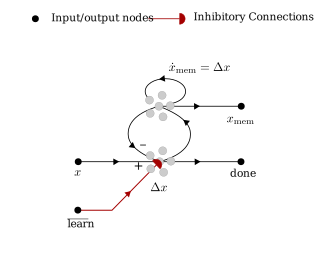
\includegraphics{media/nengo_memory_network.pdf}
	\caption{Single memory sub-network. An integrator ensemble integrates the difference between the input signal $x$ and the currently stored value $x_\mathrm{mem}$. For small difference values $\Delta x$ an output indicates that the memory is \emph{done} learning. The input $\overline{\mathrm{learn}}$ allows to stop the learning process and to maintain the currently stored value. See next page for a description.}
	\label{fig:nengo_memory_network}
\end{figure}

\begin{figure*}
	\centering
	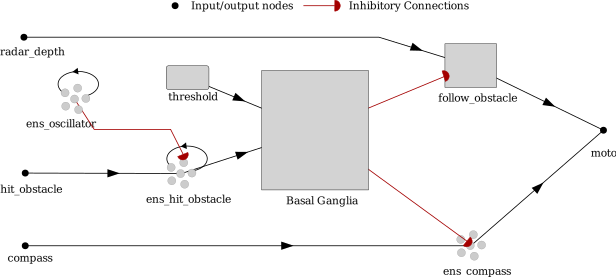
\includegraphics{media/nengo_bug_0_network.pdf}
	\caption{Sketch of the neural network implementation of Bug 0. See text on previous page for a description.}
	\label{fig:nengo_bug_0_network}
\end{figure*}

\Cref{fig:nengo_bug_0_network} sketches the network architecture used in the neural implementation of the Bug 0 algorithm. The network executes the two basic behaviours---following the obstacle outline and driving in the relative compass direction towards the goal---at the same time. The network uses a \emph{Basal Ganglia} sub-network---a circuit modelled after the Basal Ganglia in vertebrates \cite{stewart2010a}---to select one of the behaviours based on a low-passed filtered version of the contact sensor signal. This signal is periodically suppressed by a \SI{1}{\hertz} oscillator, forcing the robot to test whether it can move towards the goal. The actual behaviour selection is performed by inhibiting inactive portions of the network. An inhibitory connection is established by selecting connection weights $(W)_{ij}$ in such a way that negative currents are injected into the post-synaptic neuron ensemble, suppressing all neural activity. Due to the linear decoders in the NEF, inactive neuron populations represent the value zero.

\subsection{Implementation of Bug 2}

From the pseudo-code description of bug algorithms in \Cref{sec:background} we can deduce four possible states: \emph{(i)} memorizing the absolute orientation towards the goal at the start location, \emph{(ii)} moving towards the goal, \emph{(iii)} storing the distance to the goal upon hitting an obstacle, and \emph{(iv)} following the obstacle outline. As with the Bug 0 implementation described above, all these behaviours can be easily implemented and executed in parallel as a neural network. In comparison to Bug 0, the only new behaviour is storing values in memory. Here, I implement a simple working memory which stores values in neural activity, as opposed to long-term memory which adapts synaptic weights \cite{eliasmith2013build}. The corresponding network is depicted in \Cref{fig:nengo_memory_network}. It allows to interrupt the learning process---i.e.~to retain a value in memory---and provides a signal indicating whether learning is done---i.e.~the value stored in memory is close to the target value.

From an implementation point of view, a complication in contrast to Bug 0 is the fact that Bug 2 needs to take its current state into account when switching between behaviours. The first behaviour that needs to be executed is \emph{(i)} and following behaviours must cycle through states \emph{(ii)}-\emph{(iv)}. The present implementation solves this using a state transition network. Each behaviour provides a signal indicating whenever it is \enquote{done} (e.g.~the \enquote{move towards goal behaviour} hits a wall, the \enquote{follow obstacle outline} behaviour abortion condition is met, one of the two memories has converged to the target value), and the state transition network disinhibits the behaviour corresponding to the next state in a transition table.

\begin{figure*}
	\centering
	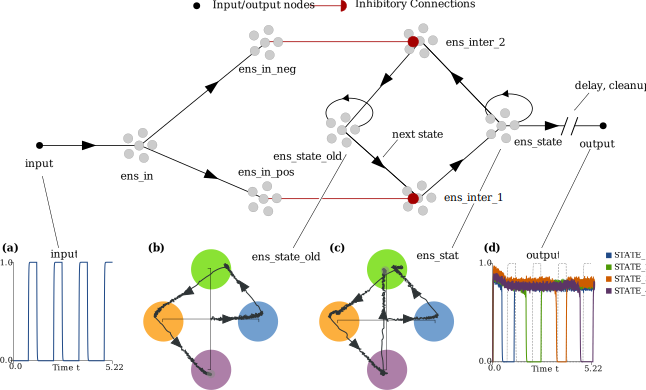
\includegraphics{media/nengo_state_network.pdf}
	\caption{Sketch of the state transition network used in the implementation of Bug 2. \textbf{(a)} exemplary input signal, \textbf{(b)} old state trajectory over time in 2D state space; coloured regions indicate state space attractors, \textbf{(c)} current state over time in 2D state space, \textbf{(d)} inverted output after cleanup and delay; high output values correspond to inactive states being inhibited. See text for a description.}
	\label{fig:nengo_state_network}
\end{figure*}
The state transition network is depicted in \Cref{fig:nengo_state_network}. In technical terms, it resembles an edge-triggered flip-flop. Whenever the input signal (the sum of all \enquote{done} signals described above) has a rising edge, the network transitions to the next state. While the input has a small value, the network transfers the current state to an \enquote{old state} ensemble. Whenever the input is high, the connection form \enquote{current state} to \enquote{old state} is inhibited and the next state is decoded from \enquote{old state} and transferred to the \enquote{current state}. States are represented as two-dimensional points on the unit-circle. The \enquote{old state} and \enquote{current state} ensembles implement attractor dynamics \cite{eliasmith2005unified,eliasmith2007attractor} to cleanly converge to one of the possible states. The four-dimensional output value is cleaned up through a low-pass filter adding additional delay, a hysteresis network preventing unwanted transient state transitions, and finally inverted, facilitating inhibition of inactive behaviours.


\section{Experiments and Results}
\label{sec:experiments}

I am comparing the neural bug algorithm implementation to a pure Python reference which---on a conceptual level---uses the same basic behaviours. In terms of resource utilization, the neural Bug~0 implementation uses a total of 2050 LIF neurons, whereas Bug~2 requires 4010 neurons.\footnote{For reference, Wikipedia lists between 250 thousand and one million (significantly more complex) neurons for the entire insect brain, see \emph{List of animals by number of neurons} (2017, July 26).}

\begin{figure}
	\centering
	\includegraphics{media/vis_traj_map_demo_03_bug_0_neural_bug_0_ref_bug_2_neural_bug_2_ref.pdf}
	\caption{Robot trajectories in an environment not solvable for Bug~0. Trajectories are similar for the corresponding reference and neural variants.}
	\label{fig:experiment_1_trajectory}
\end{figure}

\begin{figure}
	\centering
	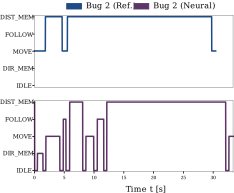
\includegraphics{media/vis_trace_map_demo_03_bug_2_ref_bug_2_neural.pdf}
	\caption{State over time for the Bug~2 trajectories shown in \Cref{fig:experiment_1_trajectory}. The reference implementation is faster due to the lack of a memorization phase.}
	\label{fig:experiment_1_states}
\end{figure}
\Cref{fig:experiment_1_trajectory} shows the performance of Bug~0 and Bug~2 for an obstacle topology in which Bug~0 should fail from a theoretical perspective. Indeed, both reference and neural implementation exhibit a highly similar behaviour and do not reach the goal. Instead, and as elaborated in \Cref{sec:background}, they continue to repeat the same trajectory over and over again. While the neural and reference Bug~2 implementations clearly do not find the shortest path from start to goal, both reach the goal and as with Bug 0, their trajectories are highly similar, even though slight differences in velocity exist. As shown in the state-over time plot in \Cref{fig:experiment_1_states}, the neural implementation requires significant time to memorize the angles and directions, whereas this process is practically instant on a traditional computing substrate.

\begin{figure*}
	\centering
	\includegraphics{media/vis_traj_map_02b_bug_0_neural_bug_0_ref_bug_2_neural_bug_2_ref.pdf}
	\caption{Robot trajectory in a large environment. Dotted line shows the shortest path assuming a point robot. Three out of eight neural Bug 2 robots reach the goal, the rest endlessly circles obstacles. Both neural and reference Bug 0 robots reach the goal on a highly similar path, yet their trajectory is significantly longer than the reference Bug 2 trajectory.}
	\label{fig:experiment_2_trajectory}
\end{figure*}
\Cref{fig:experiment_2_trajectory} shows a similar experimental setup with a larger map (causing, due to normalization, a reduced resolution for distances and angles) and eight instances of the neural Bug~2. Here, both Bug~0 (neural and reference implementation), as well as the reference implementation of Bug~2 reach the goal, where the reference Bug~2 trajectory is relatively close to the shortest path. Only one instance of the neural Bug~2 closely follows this path, and a total of five instances are stuck in circles around obstacles. Collision with those obstacles is caused by the robots leaving previous obstacles at a point not exactly on the connecting line between start and goal location due to imprecision in the direction representation. This causes a collision with an obstacle that does not have any intersection with the start-goal line at all. Correspondingly, the affected robots are---at least in theory---not allowed to leave. In practice however, noise and emergent chaotic dynamics may cause the robot to leave the obstacle outline after a few cycles. In contrast, in one case the robot never leaves an obstacle outline which clearly intersects the start-goal line. Further analysis shows that for some reason the neuron ensembles representing state in the state transition network of this instance do not fully converge to the new state, and due to attractor dynamics, the network converges back to the original obstacle-following behaviour.

To summarize, the prototypical implementations suggests that it is \emph{in principle} possible to implement Bug algorithms as neural networks. Especially the results for Bug 0 are basically indistinguishable from the reference implementation. For Bug 2, issues remain with larger maps reducing precision, as well as a lack of fine-tuning of the network dynamics and noise causing (or preventing) switching behaviours at the correct moment in time.

\section{Conclusions and Future Directions}
\label{sec:conclusion}

I presented a neural version of two basic local navigation policies, namely the \emph{Bug 0} and \emph{Bug 2} algorithm. To this end, I implemented a robot simulator which executes behaviours specified as imperative programs or spiking neural networks. Experiments show that it is clearly possible to realize the aforementioned algorithms on a neural computing substrate with relatively few neurons, assuming the presence of a corresponding sensory system. However, with increasing size and complexity of the virtual robot arena, the performance of the neural \emph{Bug 2} implementation breaks down due to inevitable imprecisions in memory and sensor processing, questioning the biological plausibility of both the provided implementation and the algorithm itself.

Even assuming that biological sensor systems exist which map onto the theoretical one---e.g.~some evidence suggests insect antennas being capable as olfactory direction sensing if a steep chemical gradient exists \cite{schneider1964insect}---the provided implementation is not a model in a strict sense, since it does not possess any predictive power concerning actual insect behaviour. With some squinting, behavioural patterns corresponding to Bug 0 can be found in insects. E.g.~meticulous research by Wehner et al.~shows that desert ants of genus \emph{Cataglyphis} use an odometer for distance measurements, sky polarisation for orientation, and their visual system for landmark navigation when returning to their nest \cite{wehner1995pathintegration,wehner2003desert,wehner2004distance}. However, there are far to many seemingly random components in insect behaviour that contradict the carefully laid out sequence of actions in the Bug 1 and Bug 2 policies, and even \emph{Cataglyphis} resorts to a randomly looking search strategy when its path is obstructed. To conclude, bug algorithms may be too restrictive on the one hand---e.g.~insects are capable of using a visual system for orientation and can store more than two variables---but require too high precision on the other hand, e.g. leaving the obstacle outline on \emph{exactly} the intersection line between the start and the goal location in the Bug 2 algorithm.

Future research should focus on more extensive experiments, e.g.~performing experiments with varying neuron count, adapting the bug policies to require less precision (better noise resilience), and incorporating results form biological studies on insect and animal navigation behaviour in general, as well as already published insect-inspired algorithms \cite{moller2012model}. Not only may this lead to more biologically plausible, but also to more robust algorithms which can be employed in neurorobotics.


%%%%%  

% Here we include the bib files 
\printbibliography

\end{document}
